% How to implement the deterministic threads.
\Dthreads{} is built on \Sheriff{} framework to support deterministic executions of
multithreaded programs:  a program with the same input always has the same execution and 
the same output.
\Dthreads{} is also a drop-in replacement of the \pthreads{} library:
users don't need to change their programs, 
to recompile their programs, nor to change the underlying operating
systems. \dthreads{} automatically provides the determinism for programs if they are linked to 
\dthreads{} library directly or using LD\_PRELOAD mechanism.

To support the deterministic running of a program, 
\Dthreads{} breaks the whole execution into intermittent parallel phases and serial phases 
(see Figure~\ref{fig:dthreadsphases}) based on explicit synchronization calls of a program: 
program sections without synchronizations are running in parallel 
phases and others are running in serial phases.
Synchronizations are those ways to communicate across different threads, 
including thread creation and exit; mutex lock and unlock; conditional variable wait
and signal; posix sigwait and signal; and barrier wait. 

In parallel phases, thread executions are running in the isolation mode, which is discussed 
in detail in Section~\ref{sec:dthreadsisolation}.
In serial phases, updates from different threads are exposed to other threads 
in a deterministic order and deterministic synchronizations are performed, which are 
discussed in Sections~\ref{sec:dthreadsdeterm}. 

\begin{figure}[b]
{\centering 
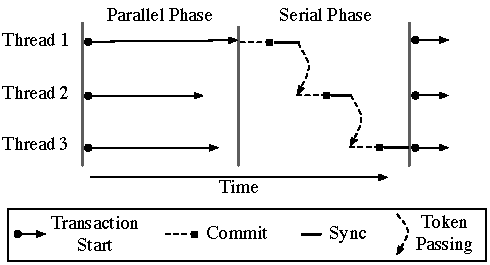
\includegraphics{dthreads/figure/phase-diagram} 
\caption{Overview of \dthreads{} phases
\label{fig:dthreadsphases}}
}
\end{figure}

\section{Isolated Memory Accesses}
\label{sec:dthreadsisolation}

\Sheriff{} framework provides a ``per-thread-isolation'' mechanism, isolating the executions
of different threads relying on different address spaces of processes.
\dthreads{} utilizes this isolation mechanism to localize different threads' modifications in
parallel phases: 
updates of each thread can not be seen by other threads and a thread can only observe those 
changes made by itself in the program order. 
Inside a parallel phase, the execution is not intervened by those executions from other threads 
so it is guaranteed to be deterministic. 

\section{Deterministic Memory Updates and Synchronizations}
%In the serial phases, updates from different threads are exposed in a deterministic order and deterministic synchronizations are performaned. We discussed these mechanisms in Sections~
\label{sec:dthreadsdeterm}
Since multithreaded programs often use shared memory to communicate, 
\dthreads{} must expose one thread's modifications 
to other threads at synchronization points deteriminically in order to ensure 
the deterministic execution.
%, these updates must be applied at deterministic times, and in a deterministic order.
%\dthreads{} exposed those modifications to the shared mapping in sequence 
%at synchronization points.
 
However, those local modificatons can not be exposed immediately when a thread reaches a 
synchronization point: committing local updates to the shared mapping should not
change the views of memory state for other threads. 
In order to guarantee the determinism, \dthreads{} introduces an internal fence: 
a thread only commits its local modifications after all other threads reach 
the same internal fence. 
This fence is similar to the barrier mechanism of \pthreads{}.  
We re-implemented this since
\pthreads{} barrier can not support the change of waiters number dynamically.

In order to avoid races in commit procedures, those commits must be performed in a 
deterministic order: 
\dthreads{} invents a global token to pass across differnt threads in a round-robin way  
and a thread can only commit its local modifications when holding the token.

The order to pass token is set to the order of threads creation initially but can be changed 
in some cases: 
when a thread is waiting on conditional variables, this thread will be taken out of the list 
of token passing; it will be put to the list again when waken up from conditional wait. 
Also, synchronizations are performed by utilizing this global token too: a thread can perform 
synchronizations when it holds the token. 

It is possible to encounter the deadlock problem when a thread holding multiple locks 
performs locks one by one using this global token. 
\dthreads{} treats multiple locks as a single lock: the token is passed to next thread when all locks
are released. 

\section{Conclusion}

Comparing to previous deterministic multithreading, 
\Dthreads{} provides a stable deterministic multithreading even in
the faces of data races: executions of a program always behave the same, even with different inputs or 
on different hardware, as long as the synchronization order is staying the same. \Dthreads{} 
dramatically improves the performance of the state-of-the-art (CoreDet~\cite{coredet}) by
3.4$\times$ without resorting to any hardware change.
In this work, \dthreads{} novelly implements a deterministic memory allocator, which can
guarantee the determinsim even for programs with memory errors, such as buffer overflows.  

However, \dthreads{} suffers from the same shortcoming as that of \sheriff{}: those programs
with ad hoc synchronization may not work properly since \dthreads{} does not commit 
those modifications of ad hoc synchronization, which needed by synchronization, 
without explicit instrumention and annotation.
\dthreads{} can also suffer the load imbalance problem of explicit synchronization 
points of programs, 
which can still guarantee the determinism but may compromise the performance.
%\coreDet{}:. 

% Why it is performing well.
% Deterministic memory allocation. 
% What is the shortcoming: can't work for the ad-hoc synchronization. The performance may encounter the 
% load-balance problem. 
